

\documentclass[]{article}
\usepackage{graphicx}
\usepackage{amsmath}
\usepackage{amssymb}
\usepackage{amsfonts}
\usepackage{fancyhdr}
\usepackage[headheight=65pt,tmargin=150pt,headsep=95pt]{geometry}
\usepackage{ragged2e}
\usepackage{array}
\usepackage{tabularx}
\usepackage{multirow}
\usepackage{booktabs}


%list of images
\graphicspath{{./images/}}

\pagestyle{myheadings}
\markright{Extra Solar Lab Report\hfill 2663452m\hfill 16/1/2023\hfill}

\title{\textbf{Identifying Extra Solar Planets and their Key Features using 
the Doppler Wobble and Planetary Transits Methods}}
\author{2663452m (University of Glasgow)}
\date{16/1/2023}






\begin{document}
\maketitle

\begin{abstract}
This is the abstract

\end{abstract}
\newpage


% All relevant sections for Method 1 (Doppler Wobble)

\twocolumn
\section*{Introduction and Background}
The search for extra-solar planets has been a growing field of Astronomy for the 
past 30 years since the first extra-solar planet was discovered in 1992, this 
detection was made indirectly by observing gaps in a pulsars emission of radio waves.$^1 $
However it wasnt until 1995 that the first direct detection of an extra-solar planet 
via the radial velocity method was made.$^2$ This method is based on measuring the 
wavelength and intensity of light emitted from a star over a period of time, 
from this, a pattern can be seen where when the star is moving towards the observer
the wavelength of the light emitted is shifted towards the blue end of the 
Electromagnetic spectrum 
(resulting in a lower wavelength) and when the star is moving away from the observer
an increase in wavelength is observed (redshift). 
\par
By measuring the wavelength and intensity and thus the radial velocity of a star as 
a function of time, it is possible to determine characteristics about the Planetary
companions in orbit such as the mass of the planet using Kepler's third law and Newton's
law of Unviersal Gravitation, an equation can derived as seen in equation 1.$^3$
\begin{equation}\label{eq:mass of planet eq}
  v_s = \left(\frac{2\pi G}{T}\right)^{1/3}M_s^{-2/3}m_p
\end{equation}
where $v_s$ is the amplitude of the radial velocity curve (RVC), $G$ is the unviversal
gravitational constant, $T$ is the orbital period of the planet, $M_s$ is the mass of
the star and $m_p$ is the mass of the planet.
\par
From the mass of the planet the semi-major axis of the orbit of the planet can be 
calculated using Kepler's third law as seen in equation 2.$^3$

\begin{equation}\label{eq:semi-major axis eq}
  G(M_s+m_p) = \frac{4\pi^2a^3}{T^2}
\end{equation}
where $a$ is the semi-major axis of the orbit, $G$ is the unviversal gravitational
and the rest of the variables are the same as in equation 1.
\par



\section*{The Doppler Wobble Method of extra-solar planets}
\par
For the analysis on data of two stars and the existence of an extra-solar planets 
around them, the doppler wobble method was used. This method is based on measuring the 
radial velocity of the stars (HD-28185 and HD-73256) as they move towards and away from 
the observer. Thus
producing a doppler shift in the light emitted from the stars, that can be used to 
determine the velocity of the stars in the plane of the observer's line of sight. 
\par
To determine the radial velocity, observations were made of the stars on different
Julian dates, recording the wavelength of light emitted as well as the observed intensity 
of the light. The radial velocity of the stars can then be calculated using the doppler
shifted wavelength and intensity, as provided in the Python Library.$^3$ 
\begin{equation}\label{eq:wavelength doppler}\lambda_{obs} = \lambda_{emit}{(1+v/c)}
\end{equation}

\begin{equation}\label{eq:intensity doppler}I_{obs} = \frac{I_{emit}}{(1+v/c)}
\end{equation}
where $\lambda_{obs}$ is the observed wavelength, $\lambda_{emit}$ is the 
emitted wavelength, $I_{obs}$ is the observed intensity, $I_{emit}$ is the emitted 
intensity, $v$ is the radial velocity of the stars and $c$ is the speed of light.
From this it was possible to calculate the radial velocity of each star on each date.
This was done using the Python SCIPY library.$^4$ An uncertainty in the radial velocity
was assigned to each date of each star of $\pm 15 ms^-1$.$^3$
\par

\begin{figure}[h]
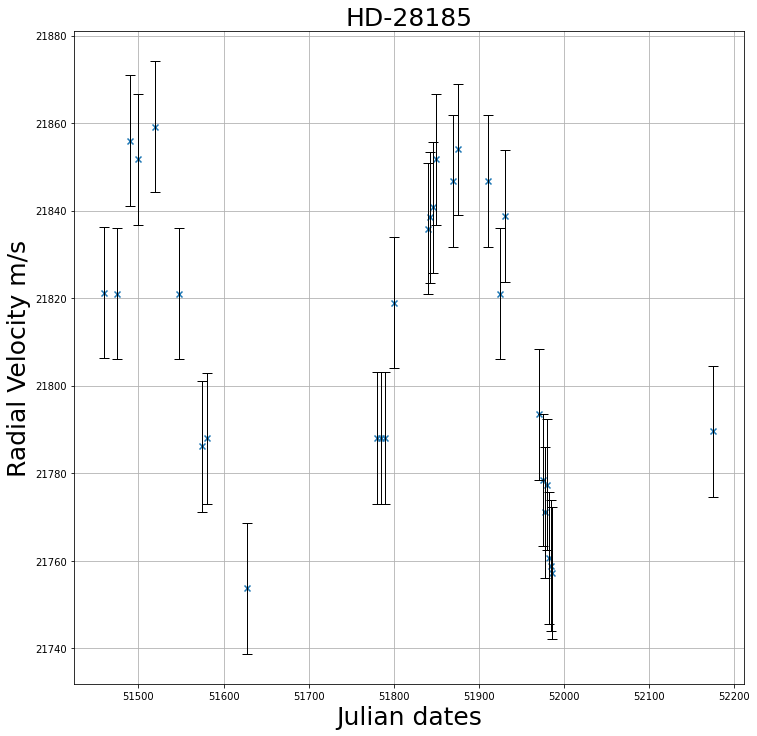
\includegraphics[width=6cm]{images/HD-28185_init.png}
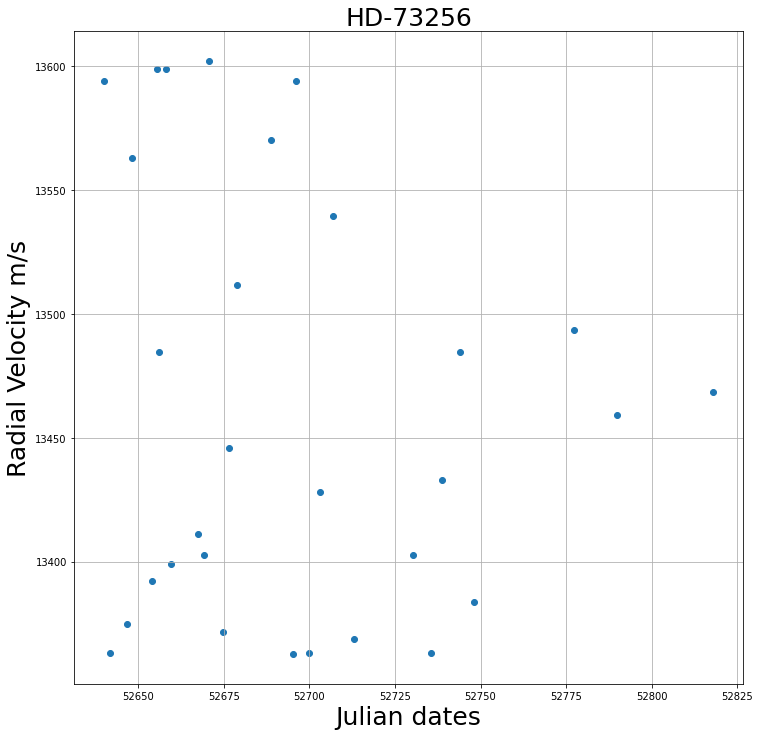
\includegraphics[width=6cm]{images/HD-73256_init.png}
\caption{Radial velocity of HD-28185 and HD-73256 as a function of time (Julian Date)}
\label{fig:HD-_init}
\end{figure}

When plotting the radial velocity as a function of time, as seen in figure 1, it was
possible to see that there was a periodic sinusoidal pattern in the data, however, 
it was not very accurate as the time between observations varyed.
To correctly plot the radial velocity of the stars over time it was neccessary 
to calculate the phase of each star through the period of the orbit. In this experiment
the phase is defined as the fraction of the orbital period that has elapsed.
The radial velocity of the stars (HD-28185 and HD-73256) as a function of phase 
was then plotted, as seen in figure 2. This allowed for a more accurate representation
of the radial velocity of the stars as a function of time, as the time between 
observations was more consistent.
\par
\newpage

\begin{figure}[h]
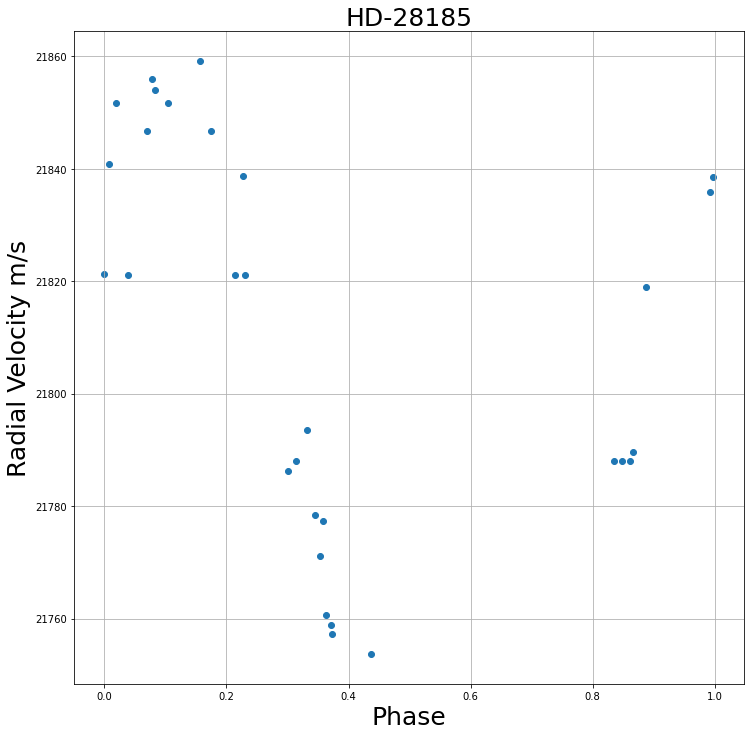
\includegraphics[width=6cm]{images/HD-28185_phase.png}
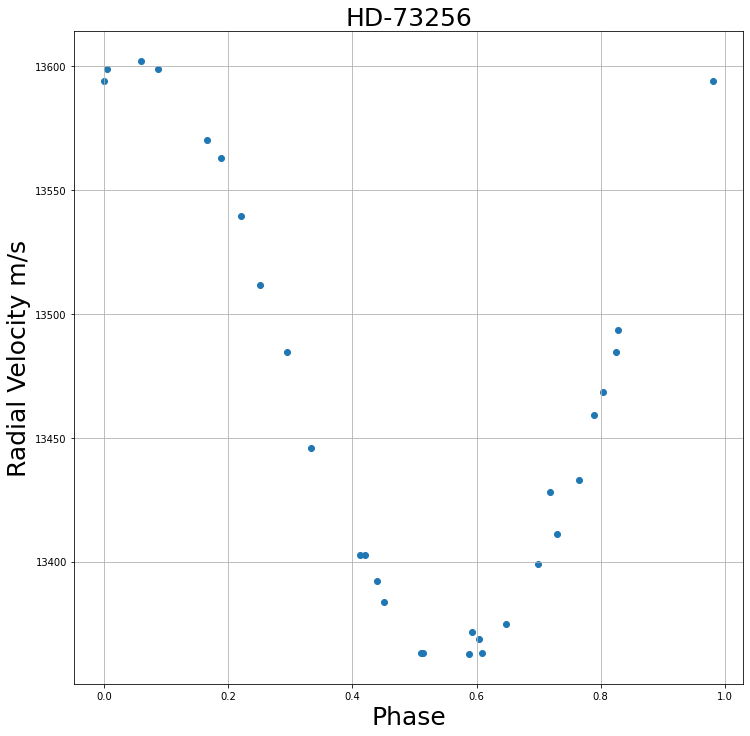
\includegraphics[width=6cm]{images/HD-73256_phase.png}
\caption{Radial velocity of HD-28185 and HD-73256 as a function of phase}
\label{fig:HD-_phase}
\end{figure}

Now that there was a clear correlation between the radial velocity of the stars and
time, it was possible to calculate characteristics about the extra-solar planets in 
orbit around the stars (HD-28185 and HD-73256) using %equation 2 from lab script. 
By using the data calculated so far in this report it was possible to now calculate 
the mean radial velocity $v_{mean} $, the amplitude of the (RVC)
 $v_{s}$ and the 
phase when the RVC is at a maximum $\phi_{max}$ of the stars.
As well as the associated covariance matrix uncertainties for each of these values.
\par
For the stars (HD-28185 and HD-73256) the values obtained for $v_{mean}$, $v_{s}$ 
and $\phi_{max}$ were.


\begin{table*}[t]
    \begin{center}
      \caption{Radial velocities and Phase of stars HD-28185 and HD-73256.}
      \label{tab:table1}
      \begin{tabular}{c|c|c}
         & {HD-28185} & {HD-73256} \\
        \hline
        $v_{mean} $ & $ 2.18\times10^4 \pm4.00ms^{-1}$ & $1.35\times10^4\pm2.80ms^{-1}$ \\
        \hline
        $v_{s}$ & $67.6\pm6.16ms^{-1} $ & $1.20\times10^2\pm3.92ms^{-1}$\\
        \hline
        $\phi_{max}$ & $8.59\times10^{-2} \pm 0.01$ & $5.73\times10^{-2}\pm0.01$  \\
        
      \end{tabular}
    \end{center}
  \end{table*}
\begin{table*}[t]
    \begin{center}
      \caption{Mass and semi-major axis of planets in orbit around stars HD-28185 and HD-73256.}
      \label{tab:table2}
      \begin{tabular}{c|c|c}
         & {HD-28185} & {HD-73256} \\
        \hline
        $m_p$ & $1.7654\pm0.1089\times10^{25}kg$ & $1.0517\pm0.0413\times10^{26}kg$ \\
        \hline
        $a$ & $2.2756\pm0.1365\times10^{6}m$ & $2.5446\pm0.1018\times10^{7}m$\\
        
      \end{tabular}
    \end{center}
  \end{table*}
Values of $\phi_{max}$ are dimensionless in this instance as they are
fractions of the orbital periods.
\par
Now that values for $v_{mean}$, $v_{s}$ and $\phi_{max}$ of both stars have 
been calculated, it was possible to determine the mass and semi-major axis of the
extra-solar planets in orbit around the stars (HD-28185 and HD-73256).
The mass of the planets was calculated using %equation 1 from the lab script.
where the mass of the planet $m_p $ is dependent on the amplitude of the RVC $v_{s}$, the mass of the star $M_s$ and the period of the orbit of the planet $T$.
As the mass of the parent star had not been calculated previously it was necessary to
make an educated assumption of what this mass might be. Therefore based on the idea 
that these stars share similar properties to the sun it was assumed that the mass of
the parent stars was $M_s = 1.0M_{\odot}$. Then using %equation 3 from the lab script
it was possible to calculate the semi-major axis of the planets in orbit around the
stars (HD-28185 and HD-73256). The values for the mass and semi-major axis of the 
relevant planets around each star are shown in table 2, with the associated 
uncertainties progated from the uncertainties in the values of $v_{mean}$, $v_{s}$
and $T$.


  \par
  


% All relevant sections for Planetary transits method
\newpage
\section*{Introduction and Background}

\section*{Aims}

Obtain a phase-folded photometric light curve for a star with a transiting 
planetary companion. Use this to estimate the radius and orbital semi-major 
axis of the planet
Apply the method of least-squares to estimate mean apparent magnitudes 
during the transit and non-transit phase. Hence estimate the radius of the planet.$^1$


\section*{Method}

\section*{Results}

\section*{Analysis}


\section*{Conclusion}

\section*{References}
\newpage

[1] {1992Natur.355..145W,
       author = {{Wolszczan}, A. and {Frail}, D.~A.},
        title = "{A planetary system around the millisecond pulsar PSR1257 + 12}",
      journal = {nat},
     keywords = {Binary Stars, Extrasolar Planets, Orbital Mechanics, Planetary Systems, Pulsars, Accretion Disks, Least Squares Method, Neutron Stars, Radio Astronomy, Supernova Remnants, Astrophysics},
         year = 1992,
        month = jan,
       volume = {355},
       number = {6356},
        pages = {145-147},
          doi = {10.1038/355145a0},
       adsurl = {https://ui.adsabs.harvard.edu/abs/1992Natur.355..145W},
      adsnote = {Provided by the SAO/NASA Astrophysics Data System}

      
}\parskip 0.2cm
\noindent
[2] Mayor, M., Queloz, D. A Jupiter-mass companion to a solar-type star. Nature 378, 355–359 (1995)
. https://doi.org/10.1038/378355a0\parskip 0.2cm

\noindent
[3] School of Physics and Astrophysics - University of Glasgow, 
Detecting Extrasolar Planets, Astronomy 2 Lab Script, 2022-2023, 9th November 2022\parskip 0.2cm

\noindent
[4]{2020SciPy-NMeth,
  author  = {Virtanen, Pauli and Gommers, Ralf and Oliphant, Travis E. and
            Haberland, Matt and Reddy, Tyler and Cournapeau, David and
            Burovski, Evgeni and Peterson, Pearu and Weckesser, Warren and
            Bright, Jonathan and {van der Walt}, St{\'e}fan J. and
            Brett, Matthew and Wilson, Joshua and Millman, K. Jarrod and
            Mayorov, Nikolay and Nelson, Andrew R. J. and Jones, Eric and
            Kern, Robert and Larson, Eric and Carey, C J and
            Polat, {\.I}lhan and Feng, Yu and Moore, Eric W. and
            {VanderPlas}, Jake and Laxalde, Denis and Perktold, Josef and
            Cimrman, Robert and Henriksen, Ian and Quintero, E. A. and
            Harris, Charles R. and Archibald, Anne M. and
            Ribeiro, Ant{\^o}nio H. and Pedregosa, Fabian and
            {van Mulbregt}, Paul and {SciPy 1.0 Contributors}},
  title   = {{{SciPy} 1.0: Fundamental Algorithms for Scientific
            Computing in Python}},
  journal = {Nature Methods},
  year    = {2020},
  volume  = {17},
  pages   = {261--272},
  adsurl  = {https://rdcu.be/b08Wh},
  doi     = {10.1038/s41592-019-0686-2},
}
\end{document}